%\documentclass[11pt]{article}
%\usepackage[utf8]{inputenc}
%\usepackage{amsmath}
%\usepackage{coling2018}
%\usepackage{todonotes}
%\usepackage{natbib}
%\usepackage{url}

\chapter{Revisiting the Hierarchical Multiscale LSTM}
%\author{Ákos Kádár \\
%	Tilburg University \\
%   {\tt a.kadar@uvt.nl}\\\And
%   Marc-Alexandre Côté \\
%   Microsoft Research Montreal\\
%      {\tt macote@microsoft.com} \\\AND
%      Grzegorz Chrupała\\
%      Tilburg University \\
%      {\tt g.chrupala@uvt.nl } \\\And
%      Afra Alishahi\\
%      Tilburg University \\
%      {\tt a.alishahi@uvt.nl}\\
%}

%\begin{document}

\section{Pre-amble}
This Chapter comprises of two parts: 1.) this pre-amble, which gives the reader context about the article and its relationship to the other parts of the thesis and some 
negative results, 
2.) a reproduction study of the Hierarchical Multisale LSTM (HMLSTM) architecture published at COLING 2018, presented after this pre-amble.

The authors originally
aimed at applying the HMLSTM architecture to learning visually grounded representations from the character level. It is a particularly
intriguing architecture for the task as it learns interpretable multi-level segmentation of the input string presented 
left-to-right through discrete boundary variables. However, we observed a considerable difficulty re-implementing the 
architecture due to the large degrees of freedom in implementation details. 
Furthermore, while the HMLSTM does converge on word-level, it does not on character level.
This we have found worrying as the comparable three-layer LSTM architecture does converge to a good solution 
and the original paper by \citep{chung2016hierarchical}
suggests that the HMLSTM should learn tasks that LSTMs learn. Rather, than abandoning 
the project we have decided to report our image-sentence ranking results here in and include a full Chapter on reproduction instead.
In the following article below we raise several points about the importance of reproducibility and verifying claims. 
Furthermore, we point to general issues when
considering complex deep-learning architectures with non-trivial implementation details and training schemes.

Here, let us present our results on image-sentence ranking using the code-base we used for the reproduction experiments. We consider
the same task as in Chapters~\ref{ch:COLI}, \ref{ch:IJCNLP} and \ref{ch:ConLL}. We learn a joint-embedding space mapping corresponding
image-sentence pairs close together. 
In all experiments we use 1024 hidden units and 300 dimensional word embeddings. Models are optimized with Adam and early stopping using 
the developement set with patience of three epochs. 
The training-objective is identical to one presented in Chapter~\ref{ch:IJCNLP}: it pushes contrastive image $i$ and caption $c$
pairs far from and true pairs close to each other (see Equation~\ref{eq:sumhinge}).

\begin{equation*}
\label{eq:sumhinge}
\begin{split}
\mathcal{J}(i, c) = \sum_{<\hat{i}, c>}[\text{max}(0, \alpha - s(i,c) + s(\hat{i}, c))] \;+ \\ \sum_{<i, \hat{c}>}[\text{max}(0, \alpha - s(i,c) + s(i, \hat{c}))]
\end{split}
\end{equation*}

The experiments presented here use the COCO data set with the by now standard splits from \cite{karpathy2015deep}. All models are 
trained on the training set, early stopping is performed on the developement set and all results are reported on the one thousand 
image test set.
The word-level results are
reported in Table~\ref{tab:hmlstmfail}. For comparison we report a comparable state-of-the-art model: VSE++ \cite{faghri2017vse++}.
The results show that all architectures get fairly close to the state-of-the-art results on word-level. Furthermore, we inspected
the internal dynamics of the HMLSTM and found that the it did learn the desired hierarchical-multiscale dynamics as indicated by the 
much lower segmentation frequency of the second layer: it segments 0.2\% of the times in layer two, which goes up to 14.5\% in layer one.


\begin{table}[]
    \centering
	    \begin{tabular}{lcccccccc}
			& \multicolumn{4}{c}{Caption Retrieval}  & \multicolumn{4}{c}{Image Retrieval} \\
		    & R@1 & R@5 & R@10 & Med r & R@1 & R@5 & R@10 & Med r \\				            
		    LSTM & 38.1  & 72.7 &  84.1 &  2.0 & 28.8 & 65.3 & 79.8 & 3.0 \\
			3-LSTM & 38.0 & 69.6 & 81.6 & 2.0 & 29.5 & 65.3 & 80.3 & 3.0 \\
			HMLSTM & 34.6 & 70.3 & 81.9 & 3.0 & 27.1 & 64.3 & 78.8 & 3.0 \\
			VSE++ & 43.6 & 74.8 & 84.6 & 2.0 & 33.7 & 68.8 & 81.0 & 3.0
		\end{tabular}
		\caption{Results on the 1K test-images of COCO on word-level.}
	\label{tab:hmlstmfail}
\end{table}

Now let us turn to the character-level results in Table~\ref{tab:hmlstmfailchar}. The one layer LSTM architecture, as expected, performs 
considerably worse on character-level than on word-level. On the other hand, the architecture with three-layers performs on par with our
best word-level model. Lastly, the HMLSTM did not converge. We tried a couple of tricks such as layer-normalization, different learning-rates,
residual connections between layers, residual connections over time and more. 

\begin{table}[]
    \centering
	    \begin{tabular}{lcccccccc}
			& \multicolumn{4}{c}{Caption Retrieval}  & \multicolumn{4}{c}{Image Retrieval} \\
		    & R@1 & R@5 & R@10 & Med r & R@1 & R@5 & R@10 & Med r \\				            
		    LSTM & 34.2  & 69.3 &  80.1 &  3.0 & 26.9 & 62.7 & 76.6 & 3.0 \\
			3-LSTM & 39.0 & 71.6 & 83.5 & 2.0 &  30.5 & 66.8 & 80.6 & 3.0 \\
			HMLSTM & 0.1 & 0.3 & 0.4 & 2491.0 & 0.1 & 0.5 & 1.0 & 500.0\\
		\end{tabular}
		\caption{Results on the 1K test-images of COCO on character-level.}
	\label{tab:hmlstmfailchar}
\end{table}


This concludes our negative results on character-level image-sentence ranking with the HMLSTM architecture. Using the same code-base
comparable architectures reached good performance, while we failed to find a setting where the HMLSTM starts to converge. 
In the following we present our reproduction study of the HMSLTM architecture as originally applied to language modeling.

\paragraph{Abstract}
Hierarchical Multiscale LSTM \citep{chung2016hierarchical} is a state-of-the-art language model that learns interpretable structure from character-level input. Such models can provide fertile ground for (cognitive) computational linguistics studies. However, the high complexity of the architecture, training procedure and implementations might hinder its applicability.  We provide a detailed reproduction and ablation study of the architecture, shedding light on some of the potential caveats of re-purposing complex deep-learning architectures. We further show that simplifying certain aspects of the architecture can in fact improve its performance. We also investigate the linguistic units (segments) learned by various levels of the model, and argue that their quality does not correlate with the overall performance of the model on language modeling. 
%\blfootnote{
%    This work is licensed under a Creative Commons 
%    Attribution 4.0 International License.
%    License details:
%    \url{http://creativecommons.org/licenses/by/4.0/}
%}

\section{Introduction}
%\todo{In experimental sciences there is a difference between reproduction and replication. Do we need to address this? GC}
%\todo{I'm not sure if that this distinction is really relevant in our community. AA}
Verifying and reproducing claims published in scientific articles is an 
essential part of building a solid foundation for future research. As such, 
reproduction has a long history in many scientific fields 
\citep{willett1985reproducibility,venables1993respiratory,
waltemath2011reproducible}. 
Recent large-scale studies, however, raise concerns about the reproducibility 
in a variety of areas and the potential effect of this crisis \citep{baker20161}. 
A reproduction study by the \citet{open2015estimating} estimates that only 40\% 
of research in psychology is reproducible, while \citet{begley2012drug} end 
up confirming only 11\% of preclinical cancer studies. The latter work makes 
an important link between the low reproducibility rates and the notoriously 
low impact of preclinical cancer research on clinical practice 
\citep{hutchinson2011high}.  

Our work is motivated by a similar concern, specifically the applicability of 
complex deep learning architectures for computational 
(cognitive) linguistics research. State of the art systems often employ complex 
architectures which integrate various design features and use many optimization
techniques. Because the focus is on boosting the final performance on a given 
task, often little effort is put into understanding where the power of the 
system comes from. This makes these models much harder to adapt for new tasks or 
domains. In our view, it is essential not only to be able to reproduce reported 
results, but also to understand the contribution of various design features through systematic ablation experiments.

%The second goal of the current study is to contribute to the interpretability of such models. 
The higher performance brought by modern neural network architectures often 
comes at the cost of our understanding of the representations and structural 
information the system learns. However, for models to be generalizable to new 
domains, it is important to move towards analyzing such structural 
representations, and investigating their impact on the final performance of 
the model.

In the current study, we examine the reproducibility of a 
language model with the ability to learn explicit linguistic structure: the 
Hierarchical Multiscale Recurrent Neural Network  (HMLSTM) model. This 
architecture was introduced by \citet{chung2016hierarchical} and set a 
new state of the art on language-modeling benchmarks Text8, Hutter Prize 
and character-level Penn Treebank. Additionally, the paper features 
examples where the lowest layer of the model recovers word-level segmentation
and in some cases performs interpretable morphological analysis. 
%Through this 
%reproduction study we examine the feasibility of re-using this type of 
%architecture, and repurposing it for tasks other than language modeling. 
With this reproduction study our motivation is to provide insight into the
dynamics of the model, which can facilitate re-using and further 
developing its architecture and repurposing it for tasks other than 
language modeling. Crucially, we investigate whether the performance of the model 
depends on the acquisition of high-quality linguistic structure.



%\todo{At this point we are not sure if we will have anything to say about the datasets, or if we have any extra tasks to report.}

\subsection{The importance of reproducibility}

There is no established tradition of reproduction studies in 
computational linguistics; however, scattered attempts at reproducing a 
number of studies have highlighted the importance of investigating the 
dataset, the model architecture and the evaluation scheme used in 
experimental designs.  For example, \citet{mieskes2017quantitative} 
quantifies the availability of non-benchmark datasets underlying the
experiments. \citet{horsmann2017lstms} re-run coarse-grained
multilingual part-of-speech tagging experiments by
\citet{plank2016multilingual} and confirm the superior performance of
LSTM-based architectures on fine-grained tagsets. 
\citet{marrese2017replication} fail to reproduce the results of three
articles in the domain of aspect-based opinion mining, with the
conclusion that repeating experiments without the availability of
source code is hindered due to lack of details on pre-processing, model architecture specification and exact parameter
settings. \citet{morey2017much} replicate the results of 9 discourse parsers
trained on the RST Discourse Treebank (RST-DT)
\citep{carlson2003building} and show that most of the recent gains in
the domain are due to non-trivial differences in evaluation
methodology. 

We propose one further step in this direction: in addition to reproducing 
reported results, it is important to investigate the role the components of  
complex models play and examine their impact on the behavior of the model.
%
The HMLSTM model that we choose as our case study has many desirable properties.
However, it is fairly complex and allows for a considerable degree of freedom 
for implementation. We experimentally explore the function of architectural details 
of the HMLSTM model, as well as experiment with varying the specifics of the 
training procedure. We aim to shed light on the potential bottlenecks involved in 
re-purposing a complex deep learning sequence modeling architecture for
computational linguistics studies. 
%Inspired by previous work on reproducibility in computational linguistics, we investigate the impact of various architectural features as well as details of the experimental setup (hyperparameter setting and training procedure) on performance. 



\subsection{The importance of interpretability}

Language data, both in the form of speech and text, exhibits
hierarchical structure: characters or phonemes form morphemes and
words, which form phrases, which in turn form whole sentences. At each
level, the units are composed to build up the meaning of the sentence
at the highest level. Modern RNN architectures have been very successful 
in solving character-level NLP tasks
\citep{chung2016character,golub2016character,mikolovsubword}.
However, they do not make the learned linguistic structure explicit:
rather it can be presumed to be cryptically encoded in the states of
the hidden layers.
%
The higher performance brought by modern neural network architectures often 
comes at the cost of our understanding of the representations and structural 
information such systems learn. However, for a model to be generalizable to new 
domains, it is important to move towards analyzing such structural representations, 
and investigating their impact on the final performance of the model.

Understanding the structural information encoded in black-box neural network 
architectures has been a desired target since \citet{elman1990finding} and several studies have 
used indirect post-analysis techniques and auxiliary tasks to probe the acquired 
structure. For example, recent studies have assessed the ability of Long Short-Term 
Memory (LSTM) language models to encode subject-verb agreement 
\citep{linzen2016assessing}, analyzed the translation quality of character-level 
sequence-to-sequence models in terms of several morpho-syntactic grammaticality 
tests \citep{sennrich2016grammatical}, \cite{li2016understanding} introduce a representation erasure technique to measure the amount of contribution of input words and specific phrases to the decision of RNN-based sentiment classifiers, \cite{kadar2017representation} examine the linguistic representations of Gated 
Recurrent Unit-based architectures for image-sentence ranking, 
and \cite{chrupala2017representations} and \cite{alishahi2017encoding} analyze the linguistic 
structure learned by Recurrent Highway Network models of visually grounded 
speech understanding. 

As an alternative approach, a number of {\em white-box} architectures have been 
proposed which learn explicit representations of linguistic structure. For 
example, \cite{dyer2016recurrent} examine Recurrent Neural Network grammars 
and analyze its learned syntax \citep{kuncoro2016recurrent}. They conclude that their architecture learns a similar notion of headedness as established head-rule sets and the model learns structure similar to traditional nonterminal categories.
\cite{williams2017learning} explore the learned grammars of two state-of-the-art natural language inference models: SPINN 
\citep{bowman2016fast} and Gumbel Tree-LSTM \citep{choi2017learning}. They find that both SPINN and Gumbel Tree-LSTM have close to or worse than chance-level parsing performance on standard benchmarks. Furthermore, they note that in the case of the SPINN architecture the learned structure depends on the tuning of the model and that their findings are different from the SPINN implementation of \cite{yogatama2016learning}. They further note that consistency of the parses produced by Gumbel Tree-LSTM across multiple runs is not far off chance level. 

The Hierarchical Multi-scale LSTM architecture \citep{chung2016hierarchical} is in 
the latter class of white-box models. It is designed specifically to allow for 
learning explicit structure in data: at each layer, it predicts a binary boundary 
variable at each time-step. These boundaries correspond to an explicit, 
interpretable segmentation of the input utterance at multiple levels, which can be 
thought of as different levels of granularity in linguistic structure. 
At the same time, it reportedly has state-of-the-art performance on several 
language modeling benchmarks. As such, we believe the model 
has the potential to impact future computational cognitive linguistics studies. 
However, it is not clear whether the high performance of this model demands
the acquisition of high-quality linguistic structure from input text. Furthermore, due to 
the complex architectural design, implementation details might play a large role in the 
conclusion that can be drawn from the learned structure 
as in \cite{williams2017learning}. We examine 
the segmentation of the input characters by different versions of this model to see
whether their quality impacts the overall performance.

% \subsection{Our study}
% \todo{not sure if this section is needed anymore.}

%\subsection{Hierarchical Multiscale LSTM}

% In this paper, we present
% \begin{itemize}
% \item a detailed discussion of the HMLSTM architecture in an attempt to make it accessible for a wider audience; 
% \item an independent replication of the original experiments of \citet{chung2016hierarchical};
% \item an ablation study, considering both training hyperparameters and architectural features;
% \item {\it extra experiments on an additional dataset/a variation of the original dataset?}\todo{If we manage to include the no-space or text8 results.}
% \end{itemize}

% Our hope is that the contribution of the paper goes beyond the HMLSTM reproduction study and helps popularize similar work in the Computational Linguistics community.\todo{AA: write a stronger paragraph once we know what goes in the final version of the paper.}

\section{Hierarchical Multiscale LSTM}

Let us introduce the notations used throughout this section with the standard LSTM equations:

\begin{align}
    \tag{gates and candidate}
     \begin{bmatrix}
               \mathbf{i}_{t} \\
               \mathbf{f}_{t} \\
               \mathbf{u}_{t} \\
               \mathbf{o}_t
      \end{bmatrix} &= W\mathbf{x}_t + U\mathbf{h}_{t-1} + \mathbf{b}  \\
             \tag{cell state}
             \mathbf{c}_t &= \mathbf{c}_{t-1} \odot \sigma (\mathbf{f}_t) + \text{tanh}(\mathbf{u}_t) \odot \sigma (\mathbf{i}_t) \\
             \tag{hidden state}
             \mathbf{h}_t &= \sigma (\mathbf{o}_t) \odot \text{tanh}(\mathbf{c}_t) 
\end{align}
The input to an LSTM are the current input $\mathbf{x}_t$, previous state $\mathbf{h}_{t-1}$ and previous 
cell state $\mathbf{c}_{t-1}$. Variables $\mathbf{x}_t$ and 
$\mathbf{h}_{t-1}$ are used to compute the input gate 
$\mathbf{i}_t$,
forget gate $\mathbf{f}_t$, candidate activation $\mathbf{u}_t$ 
and output gate $\mathbf{o}_t$. 
In the second equation $\mathbf{f}_t$ and $\mathbf{i}_t$ are used to trade off the 
candidate activation $\mathbf{u}_t$ and the previous cell-state $\mathbf{c}_{t-1}$ using the element-wise multiplication $\odot$. 
This results in the current cell state
$\mathbf{c}_t$. Finally, the output gate soft-selects the 
components of $\text{tanh}(\mathbf{c}_t)$ to write to the hidden state $\mathbf{h}_t$. The function $\sigma$ refers to the sigmoid function.

\paragraph{HMLSTM --} To make the explanation of the HMLSTM architecture more straight-forward, let us first consider the bottom- and top-layer as 
they are special cases of any $\ell$-th layer. 
In addition, we provide vectorized version equations of the HMLSTM architecture which allow for batch sizes larger than 1 (see Appendix~\ref{sect:appendix:vectorized_HMLSTM}).

\paragraph{Bottom Layer --}

The bottom layer of the HMLSTM takes as input: 1) \emph{bottom-up connection}: input  at  the current time-step $\mathbf{x}_t$; 2) \emph{recurrent connection}: hidden and cell states $<\mathbf{h^1}_{t-1}, \mathbf{c^1}_{t-1}>$  and previous
boundary variable $z^1_{t-1}$ from $\ell=1$; and 3) \emph{top-down connection}: hidden state $\mathbf{h^2}_{t-1}$ from $\ell=2$. It outputs the state tuple $<\mathbf{h}^1_{t}, \mathbf{c}^1_{t}>$ and boundary variable $z^1_t$.

\begin{align}
     \begin{bmatrix}
           \mathbf{i}_{t} \\
           \mathbf{f}_{t} \\
           \mathbf{u}_{t} \\
           \mathbf{o}_t \\
           z_t
         \end{bmatrix} &= W \mathbf{x}_t + U\mathbf{h}^1_{t-1} + z_{t-1} V\mathbf{h}^{2}_{t-1} +  \mathbf{b} 
\end{align}
The activation function on $z_t$ is the hard-sigmoid followed by
the rounding operation to discretize it to $\{0, 1\}$: 
$z_t := \mathrm{round}(\mathrm{hard\_sigmoid}(z_t))$.
The top-down connection is turned on and off by $z_{t-1}$.
When the layer detects a boundary in the previous step (i.e.\ $z_{t-1}=1$), takes context from the higher layer through the top-down connection.
  After computing the activations the layer either runs a regular LSTM UPDATE or does a FLUSH of its input:

\begin{equation}
    \mathbf{c}_t = \begin{cases}  
            \mathbf{c}_{t-1} \odot \sigma (\mathbf{f}_t) + \text{tanh}(\mathbf{u}_t) \odot 
            \sigma (\mathbf{i}_t) & \mbox{if } z_{t-1} = 0  \: \: \text{(UPDATE)}\\
            \text{tanh}(\mathbf{u}_t) \odot \sigma (\mathbf{i}_t)  & \mbox{if }  z_{t-1} = 1  \: \: \text{(FLUSH)}
            \end{cases}
\end{equation}

\noindent
The final hidden state is given by the regular LSTM update
    $\mathbf{h}_t = \sigma (\mathbf{o}_t) \odot \text{tanh}(\mathbf{c}_t)$.

\paragraph{Top Layer --}
The top layer has both bottom-up $\mathbf{h}^{\ell-1}_t, z^{\ell-1}_t$ and recurrent connections $<\mathbf{h^\ell}_{t-1}, \mathbf{c^\ell}_{t-1}>$, but no top-down connection. At each step, it outputs the state tuple $<\mathbf{h}^{\ell}_{t}, \mathbf{c}^{\ell}_{t}>$:  
\begin{align}
     \begin{bmatrix}
           \mathbf{i}_{t} \\
           \mathbf{f}_{t} \\
           \mathbf{u}_{t} \\
           \mathbf{o}_t \\
         \end{bmatrix} &= z^{\ell-1}_t W \mathbf{h}^{\ell-1}_t + U\mathbf{h}^\ell_{t-1}  + b 
\end{align}
The bottom-up input $\mathbf{h}^{\ell-1}_t$ is gated by $z^{\ell-1}_t$. 
When $z_t=1$ the higher layer takes one step and performs UPDATE; otherwise it ignores the current time-step and performs COPY:

\begin{equation}
    \mathbf{c}_t = \begin{cases}  
            \mathbf{c}_{t-1} \odot \sigma (\mathbf{f}_t) + \text{tanh}(\mathbf{u}_t) \odot \sigma (\mathbf{i}_t) &
            \mbox{if } z_t = 1  \: \: \text{(UPDATE)}\\
            \mathbf{c}_{t-1} &  \mbox{if } z_t = 0  \: \: \text{(COPY)}
            \end{cases}
\end{equation}

\paragraph{Middle layers --}

The general HMLSTM layer runs all operations: UPDATE, COPY and FLUSH. It takes as input 1) \emph{bottom-up connection}: lower layer state $\mathbf{h}^{\ell-1}_t$ and boundary variable $z^{\ell-1}_t$; 2) \emph{recurrent connection}: hidden and cell states $<\mathbf{h^\ell}_{t-1}, \mathbf{c^\ell}_{t-1}>$  and boundary variable $z^\ell_{t-1}$; and 3) \emph{top-down connection}: hidden state $\mathbf{h}^{\ell+1}_{t-1}$. It outputs the tuple $<\mathbf{h}^\ell_{t}, \mathbf{c}^\ell_{t}>$ and boundary variable $z^\ell_t$:

\begin{align}
     \begin{bmatrix}
           \mathbf{i}_{t} \\
           \mathbf{f}_{t} \\
           \mathbf{u}_{t} \\
           \mathbf{o}_t \\
           z_t
       \end{bmatrix} &= z^{\ell-1}_t W \mathbf{h}^{\ell-1}_t + U \mathbf{h}^{\ell}_{t-1} + z^{\ell}_{t-1} V\mathbf{h}^{\ell+1}_{t-1}  + b 
\end{align}
The bottom-up connection is masked by $z^{\ell-1}_t$ as in
the top-layer, while the top-down connection is masked by 
$z^{\ell}_{t-1}$ as in the bottom-layer. The variables
$z^{\ell-1}_t$, $z^{\ell}_{t-1}$ determine which of the three
operations the cell runs. FLUSH is executed if the layer detects a boundary in the previous step (i.e.\ $z^{\ell}_{t-1}=1$).
If this is not the case and the lower layer does not detect a boundary, the layer runs COPY. However, if the lower layer does detect a boundary $z^{\ell-1}_t$, it runs UPDATE:

\begin{equation}
    \mathbf{c}_t = \begin{cases}  
            \text{tanh}(\mathbf{u}_t) \odot \sigma (\mathbf{i}_t) & \mbox{if } z^l_{t-1} = 1 \: \: \text{(FLUSH)}\\
            \mathbf{c}_{t-1} &  \mbox{if } z^\ell_{t-1} = 0 \: \mbox{and} \:  z^{\ell-1}_t = 0  \: \: \text{(COPY)}\\
            \mathbf{c}_{t-1} \odot \sigma (\mathbf{f}_t) + \text{tanh}(\mathbf{u}_t) \odot \sigma (\mathbf{i}_t) &
            \mbox{if } z^\ell_{t-1} = 0 \: \mbox{and} \:  z^{\ell-1}_t = 1  \: \: \text{(UPDATE)}
            \end{cases}
\end{equation}

\paragraph{Output gate --}
The output embedding $\mathbf{h}^e_t$ of the HMLSTM is computed by the following gating mechanism:

\begin{align}
g^\ell_t &= \sigma(\mathbf{w}_\ell^T [\mathbf{h}_1; \mathbf{h}_2; \mathbf{h}_3]) \\
\mathbf{h}^e_t &= \text{ReLU}(g^\ell_t W^e_\ell \mathbf{h}^\ell_t)
\end{align}

It takes states from the three layers and computes a gating value for each 
$g^1_t, g^2_t$ and $g^3_t$ using the parameter vector $\mathbf{w}^\ell$. These scalars are used to weight the  $W^e_l \mathbf{h}^l_t$
for each layer where $W^e_\ell$ is a learned parameter. 
% Is W^e\ell a scalar or a vector?
It is important
to add some mechanism to combine the activations of the three layers for language modeling as all three layers tick on a different time-scale, but the network has to generate an output at each time-step. This combined embedding $\mathbf{h}^e_t$ is then used in the final softmax layer to predict the probability distribution over the next character.


%\paragraph{Sampling} In some experiments the authors do not threshold $z$, but
%state that they sample from the Bernoulli distribution. The actual 
%implementation performs a two class gumbel-softmax trick. 

%\paragraph{Shuffled PTB} The number of steps in the Penn-Treebank is not divisible
%by 100. As a consequence the authors random crop a portion of the PTB for each
%epoch and randomly shuffle it.


\section{Experiments}

\subsection{Experimental setup}

Upon our request, the authors of the original paper shared a code base with us implementing the HMLSTM architecture and functionality to run the experiments on Penn Treebank (henceforth PTB). The code was implemented in Tensorflow version 1.1 \citep{abadi2016tensorflow}, which we ported with minimal modifications to version 1.6 to be able to run it on our system. In the default settings, the code contains $\ell^2$-norm  weights penalty term with a coefficient of $0.0005$, which we also kept fixed across experiments. Furthermore, the given source code has a special initialization strategy used for the weights matrices: until the last column vector it is initialized with orthogonal initialization with standard normal distribution. The last column vector (corresponding to the logit of $z$) is initialized with Glorot uniform initialization with $\sigma = \sqrt{\frac{6.0}{\text{fanin} + \text{fanout}}}$. Due to no initialization details in the original paper we used the initialization defaults provided in the code base for all PTB and Text8 experiments. Lastly, the authors did not refer to publicly available pre-processed versions of the datasets and we used our versions following the details of the paper. We made the following changes to the original code:
\begin{description}
\item[Baseline --] The authors report LSTM baselines for both PTB and Text8 data sets. The exact configuration of the baseline is not discussed in the paper, however, the authors do share that they implement both layer-normalization and the output module.
We train a three-layer stacked LSTM with the same hyperparamters as the HMLSTM.
\item[Layer normalization --] The original paper reports results using layer normalization \citep{ba2016layer}, which was not implemented in the code base. There are multiple options where to apply it in the case of a LSTM cell. For the HMLSTM cell we implemented it based on equations 20-22 in the paper introducing the technique \citep{ba2016layer}. Furthermore, we applied layer-norm to the input and output embedding layers since the performance of the model was found to be unstable otherwise. 
\item[Learning-rate schedule and early-stopping --] The code base did not include an implementation of the learning-rate schedule that was reported to be used in the original experiments. The learning-rate schedule reported in the paper divides the learning rate by 50 when no improvement is observed in the validation loss. In our code we monitor the validation loss at each epoch. The original code base ran the models for 500 epochs with no early-stopping and no learning-rate schedule, however, we use early stopping with patience of 4 as very small improvements are observed after reducing the learning rate four times by 50. 
\item[Evaluation --] 
We report the bits-per-character (bpc) of the trained models by computing the entropy (in base 2) of the entire test set and dividing it by the number of characters. The code did not implement the evaluation procedure and we have not found the exact details in the paper. Our implementation follows  \cite{mikolovsubword}: we use batch size of 1 and carry the states  of the recurrent model over to the following batch of 100 characters until the 
whole test sequence is processed.
\end{description}

\noindent The experimental results reported in Section~\ref{sec:results} are all using this revised 
implementation, manipulating various ablation factors as described in 
Section~\ref{sec:ablation-factors}. 
Following \cite{chung2016hierarchical}, we report results on the following two datasets. 

\paragraph{Character-level Penn Treebank --}
The smaller-scale experiments apply variations of the model on the Penn Treebank dataset 
\citep{marcus1993building} using the splits and preprocessing from \cite{mikolovsubword}. 
All models are trained with sequence lengths of 100 and batch size of 64.
Before each epoch the dataset is randomly cropped to be divisible by 100. 
The parameters are optimized with Adam \citep{kingma2014adam}
with initial learning rate of 0.002, 
which is divided by 50 if no improvement on the validation data is observed 
after a full epoch. The norm of the gradient is clipped at 1.0. For all models 
we use 512 units for all layers and 128 dimension character embeddings as 
reported in the paper.

\paragraph{Text8 --}
The Text8 dataset \citep{mahoney2011large} is extracted from Wikipedia and is 
a sequence of 100 million alphabetical characters and spaces. The 
splits used by \cite{chung2016hierarchical} correspond to the (by now standard) 
splits introduced in \cite{mikolovsubword}: first 90M characters for training, 
the next 5M for validation and the final 5M characters for testing. On this dataset 
models are trained on sequence length of 100 and batch size of 128.
The initial learning rate of Adam was set to 0.001 and we applied the 
learning-rate schedule and early-stopping strategy described before. 
The norm of the gradient is clipped at 1.0. We use 1024
units for the HMLSTM layers and 2048 output embedding units.

Like in the original paper, models are trained to minimze the log-likelihood of the training set and
the non-differentiability gap caused by the rounding operation when 
discretizing the boundary variables is solved by using the straight-through 
estimator \citep{bengio2013estimating}.


%\todo{AA: I didn't touch the following paragraph, assuming it is not up-to-date.}

%\todo{Akos: not sure if should mention any of this tensorflow/server thing with no conclusion}
%Furthermore, we examined the stability of the model's behavior across four machines. The experiment was run until the end of the first epoch on PTB. We have found that the validation bpc is stable across machines, while the frequencies of the boundary variables have a much larger variance.
%On one of our setups we did not manage to reproduce the hierarchical multiscale behavior as the lower layer ran on a slower time-scale than the higher with average frequencies 0.05 and 0.9 respectively. On all other setups the correct behavior was observed. We report our final results using our most performant P100 configuration. The complex hardware and software configurations required to run modern deep-learning experiments seem to make it important run such sanity checks when possible. Furthermore, multiple runs with the same setup resulted in slightly different validation bpc values even after fixing the random seeds. This might be due to the non-deterministic CUDA atomics reduction operations used by TensorFlow, which we did no investigate further. In summary we identified the layer-norm implementation details, the hardware/software configuration and the inherent randomness in the software stack as sources of noise that can potentially lead to different results reported here.

\subsection{Ablation factors}
\label{sec:ablation-factors}

In order to analyze the behavior of the model and the impact of its various 
architectural design features as well as evaluation settings, we manipulate 
the following factors in our experiments. 

\begin{description}

\item[Layer normalization (LN).]
As mentioned in the previous section, there was a mismatch between the 
description of the HMLSTM model in \citet{chung2016hierarchical} and 
the code base provided to us in terms of layer normalization. Therefore 
we report our experimental results both with and without layer normalization.

\item[Learning-rate schedule (Schedule).] Similarly, the paper and the
code base do not match in applying learning-rate schedule, therefore we 
report results with and without scheduling.

\item[Sensitivity to slope ($\alpha$).] Hard-sigmoid \citep{gulcehre2016noisy} 
is a piecewise linear approximation of the sigmoid function, defined as the
first-order Taylor expansion of the sigmoid around $x \approx 0$ and
clipped between the limits of the original function (0 and 1): 
$\text{max}(0, \text{min}(1,0.25x + 0.5) )$; where 0.25 is the 
slope $\alpha$. The authors describe the slope annealing trick for the 
PTB experiments and state that they start from slope 0.5 and slowly 
increase it at maximum until 2.5. We have not found details regarding 
the $\alpha$ values in other experiments, but used the default 
$\alpha=0.5$ in the code-base.  We test whether the hard-sigmoid slope 
$\alpha = 0.25$ reaches the same performance as the 
specific choice of $\alpha=0.5$. Furthermore, we gauge sensitivity to $\alpha$ using values 0.125 and 1.0.

%\paragraph{Unsegmented input} The HMLSTM can discover hierarchical multiscale structure in sequences. However, the PTB and Text8 data sets contain spaces between words, providing a strong cue to where to segment. We remove the spaces from the PTB data set and re-run the HMLSTM with the same settings as on the original PTB. The results performance is considerably worse with 1.65 bpc after 8K iterations. The LSTM baseline achieves 1.66 bpc as such the two models are much closer in performance. 


\item[COPY operation on the last layer (CopyLast).]
The code base by default, only applies the COPY operation at the 
last layer on the cell state $\mathbf{c}^{l}_t$, but not on the 
hidden state $\mathbf{h}^{l}_t$. In the latter case if the layer 
runs COPY it takes the previous cell state and applies the new 
output gate on it along with the $\mathrm{tanh}$ function 
$\mathbf{o}_t \odot \mathrm{tanh}(\mathbf{c}_{t-1})$. This is different 
from the original formulation of the HMLSTM. The main experiments 
were run with this default, but we also report the impact of changing this parameter.

\item[Top-down connection (NoTopDown).]
When the HMLSTM cell runs the FLUSH operation, it computes
the new cell-state by $\mathbf{i}_t \odot \mathbf{u}_t$ and the 
previous cell-state is dropped from the computation.
However, both $\mathbf{i}_t$ and $\mathbf{u}_t$ depend on the previous
state $\mathbf{h}_{t-1}$. As such, information from the past steps still ``leaks'' 
even at FLUSH and each layer can potentially retain enough information 
for future computations without the use of top-down connections. 
In our experiments we run the HMLSTM model with and without top-down
input to evaluate the impact of this simplification.
%and segmentation behavior. 

\item[Simpler output layer (SimplerOut).]
The hidden state of the last layer of the HMLSTM is not updated 
at every time-step and as such it computes a gated embedding 
combining the representation of all three layers to be able 
to provide a prediction for every time-step.  
Here we implement a simplification to the output layer by replacing 
it with a single affine transformation, embedding the concatenated 
hidden states: $\mathbf{h}^e_t = \text{ReLU}(W^e [\mathbf{h}_1; \mathbf{h}_2; \mathbf{h}_3])$.

\item[Alternative architecture (HMRNN).]
One of the motivations for the HMLSTM architecture in the original paper 
\citep{chung2016hierarchical} is that the hierarchical multiscale 
structure might help with the vanishing gradient problem as gradients 
are back-propagated through fewer time-steps. Here we introduce an alternative
architecture that we call HMRNN, which replaces the LSTM updates with 
simple Elman RNN recurrence. 
It is a much simpler model and it helps in understanding if the hierarchical 
multiscale structure itself is enough to alleviate the vanishing gradient 
problem, or if the LSTM-style updates are essential for the good performance. 

\begin{equation}
    \mathbf{h}_t = \begin{cases}  
             \text{tanh}(W \mathbf{h}^{l-1}_t + V\mathbf{h}^{l+1}_{t-1} ) & \mbox{if } z^l_{t-1} = 1 \: \: \text{(FLUSH)}\\
 \mathbf{h}_{t-1} &  \mbox{if } z^l_{t-1} = 0 \: \mbox{and} \:  z^{l-1}_t = 0  \: \: \text{(COPY)}\\
    \text{tanh}(W \mathbf{h}^{l-1}_t + U \mathbf{h}^{l}_{t-1}) &
            \mbox{if } z^l_{t-1} = 0 \: \mbox{and} \:  z^{l-1}_t = 1  \: \: \text{(UPDATE)}
            \end{cases} 
\end{equation}

The HMRNN architecture implements a simple formulation of the hierarchical 
multiscale intuition. In case of the FLUSH operation, it only takes as input 
the hidden state of the lower layer and the hidden state of the higher layer 
at the previous step. In case of COPY it just uses the previous hidden state. 
Finally, when running UPDATE it applies the simple Elman network update. See Appendix~\ref{sect:appendix:vectorized_HMRNN} for a vectorized implementation.

%The vectorized version is implemented as follows:

%\begin{equation*}
%\begin{aligned}[c]
%\mathrm{c}_m &= (1 - z^\ell_{t-1})  (1 - z^{\ell-1}_t) \\
%\mathrm{u}_m &= (1 - z^\ell_{t-1})   z^{\ell-1}_t \\
%\mathbf{h}_t &=  \mathrm{c}_m  \mathbf{h}_{t-1} + (1-\mathrm{c}_m)  \text{tanh}((1-\mathrm{u}_m)  \mathrm{h}_f + \mathrm{u}_m \mathrm{h}_u )) \\
%\end{aligned}
%\begin{aligned}[c]
%\mathrm{h}_f &= W \mathbf{h}^{l-1}_t + V \mathbf{h}^{l+1}_{t-1}\\
%\mathrm{h}_u &= W \mathbf{h}^{l-1}_t + U \mathbf{h}^{l}_{t-1} \\
%\end{aligned}
%\end{equation*}

%Bottom layer:
%\begin{equation}
%\mathbf{h}_t = \text{tanh}(W \mathbf{x}_t + (1-z^l_{t-1}) U \mathbf{h}^{l}_{t-1} + z^l_{t-1} \times V\mathbf{h}^{l+1}_{t-1})
%\end{equation}

%Top layer:
%\begin{equation}
%\mathbf{h}_t = (1-z^{l-1}_t) \times \mathbf{h}_{t-1} + z^{l-1}_t \times  \text{tanh}(W \mathbf{x}_t +  U \mathbf{h}^{l}_{t-1})
%\end{equation}

% In the Results section we report the performance of the HMRNN model with that of the HMLSTM model in a similar setting.

%The large gap in performance of the HMRNN and HMLSTM architectures, provides evidence that the LSTM formulation is well motivated in the 



%\begin{align}
%\alpha_1, \alpha_2, \alpha_3 &= \text{softmax}(W^a %[\mathbf{h}_1; \mathbf{h}_2; \mathbf{h}_3]) \\
%\mathbf{h}^e_t &= \sum_l \alpha_l h_l
%\end{align}
%It removes the parameter $W^e_l$ and provides easier interpretability as the $\alpha$ values correspond to proportions.
\end{description}




\section{Experimental Results}
\label{sec:results}
\subsection{Reproducing language modeling results}

\begin{table}[t]
\centering
\begin{tabular}{lll}
                        & {\bf PTB } & {\bf Text8} \\
\hline
HMLSTM reported by \citep{chung2016hierarchical}  & 1.25 & 1.29	\\
3-layer LSTM reported by \citep{chung2016hierarchical}  & 1.29 & 1.39	\\
\hline
3-layer LSTM + Schedule + LN & 1.32  &  1.37\\

HMLSTM + Schedule + LN    & 1.27 & 1.36 \\
HMLSTM + Schedule + LN + CopyLast & 1.29  &  1.36\\
%Batchnorm LSTM            & 1.32 & 1.36 \\
\hline 
\end{tabular}
\caption{Reproducing language modeling results (in bpc) on PTB and Text8 datasets. 
%The numbers in parantheses show the number of iterations for each model.
}
\label{tab:LM-reproduction}
\end{table}
%\todo{AA: Text8 iterations are missing from the table.}


We attempt to replicate the language modeling experiments of 
\cite{chung2016hierarchical} on the character level Penn Treebank 
and Text8  datasets. Table~\ref{tab:LM-reproduction} shows the 
language modeling results reported by \cite{chung2016hierarchical} 
on both datasets. It also reports results of our reproduction 
of the original experiments as described 
in the paper. This means using the HMLSTM architecture with 
layer normalization on all layers, and with learning-rate 
scheduling. Since the use of the COPY operation on the last layer is 
ambiguous and not consistent between the original paper and the 
code base, we report results both with COPY on and off.

Our most faithful reproduction of the original experiments, 
which uses the HMLSTM architecture with learning-rate schedule, 
layer normalization and COPY on the last layer, results in 1.29 bpc 
on the PTB dataset. Dropping the COPY
option improves the results to 1.27 bpc, which is still below 
the results reported in \cite{chung2016hierarchical} on the 
same dataset (1.25). Our 3-layer LSTM baseline on PTB also under performs the baseline reported by \cite{chung2016hierarchical}(1.32 compared to 1.29 bpc).

On the Text8 dataset, our results (1.36) are 
much further from the published ones (1.29), with the HMLSTM performing very close to
the 3-layer LSTM baseline (1.37).
We did not pursue further experiments on this dataset. 
The discrepancy could be due to the fact that the script that 
the authors shared with us was optimized for PTB, and some of 
the settings might need to be changed for Text8. However, 
since we have not found such differences reported in the paper, we used the same setting for both datasets.
Interestingly, contrary to the HMLSTM results, our implementation of
the 3-layer LSTM basline improves the reported baseline performance from 1.39 to 1.37 bpc.

\subsection{Ablation results}

% Results on the P100 using commit >=
% b98555fe9473a2831939461940543118e8833a4d
\begin{table}[ht]
\centering
\begin{tabular}{lllcccc}
                        & & BPC & Iter. & $z^1$ & $z^2$ & $z$-ratio\\
\hline 
\hline
1 & HMLSTM + Schedule + LN + copylast      & 1.29   & 10K & 0.41 & 0.25 & 1.64 \\
\hline 
2 & HMLSTM                  & 1.39   & 16K	& 0.23 & 0.15 & 1.53 \\
3 & HMLSTM + Schedule      	& 1.32   & 12K	& 0.25 & 0.16 & 1.56\\
4 & HMLSTM + Schedule + LN  & 1.27 & 12K  & 0.42 & 0.09 & 4.67 \\
\hline 
% NB: The alpha corresponds to the value for --alpha in our code.  
5 & HMLSTM + Schedule + LN + $\alpha$=0.125 & 1.28  & 14K & 0.41 & 0.23 & 1.78\\
6 & HMLSTM + Schedule + LN + $\alpha$=0.25  & 1.27  & 12K & 0.31 & 0.21 & 1.48 \\
7 & HMLSTM + Schedule + LN + $\alpha$=1.0    & 4.32  &  4K & 1.0 & 1.0 & 1.0 \\
\hline 
8 & NoTopDown + Schedule + LN  		&  1.28 & 12K & 0.64 & 0.28 & 2.29\\
9 & SimplerOutput + Schedule + LN   &  {\bf 1.25}    & 10K & 0.64 & 0.31 & 2.06 \\
\hline 
%10 & Batchnorm LSTM          & 1.32 & 	~	 &   ~   &   ~   \\
10 & 3-layer LSTM + Schedule + LN   		       &  1.32    & 9K & N/A & N/A & N/A\\
11 & 3-layer LSTM + Schedule + LN + SimplerOut &  1.26    & 12K & N/A & N/A & N/A\\
12 & HMRNN + Schedule + LN   		&  1.40    & 18K & 0.0 & 1.0 & 0.0\\
\hline 
\hline 
\end{tabular}
\caption{Ablation results on PTB}
\label{tab:ablation}
\end{table}

Since we did not succeed in reproducing the original results 
on Text8, we only perform the ablation experiments on the 
PTB dataset. Table~\ref{tab:ablation} summarizes the results 
of these experiments. On the first row, we repeat our reproduction 
results using the most faithful replication of the original 
experiments (HMLSTM + Schedule + LN + CopyLast). We will 
compare the results from various modifications of the 
architecture or evaluation setup to these base results.

\paragraph{Layer normalization and learning-rate schedule --} 
As is evident from the results on rows 2--4, adding 
learning-rate schedule and layer normalization improve 
the results over the base HMLSTM. Furthermore, the 
results on row 4 (HMLSTM + Schedule + LN) are better 
than the reproduction results which also implement the 
CopyLast feature. Therefore, in the rest of the experiments, 
we consistently add layer normalization on all layers as 
well as learning-rate scheduling, and drop CopyLast.

\paragraph{Sensitivity to alpha --}
Rows 5--7 show results for different values of the slope 
$\alpha$. Using the by definition hard-sigmoid slope $\alpha=0.25$ 
instead of the default $\alpha=0.5$ in the code does not degrade 
the performance. Lowering alpha to $\alpha=0.125$ degrades 
the performance slightly. Since \cite{chung2016hierarchical} 
mention that they increase the slope up to $\alpha=2.5$, we 
also tested the results with a higher value of $\alpha=1.0$ (row 7), 
which caused the model to diverge after 4,000 iterations.

\paragraph{Architectural modification: top-down connection and simpler output --} Interestingly, as can be seen from row 8, removing the top-down 
connections (and keeping the model structure fixed otherwise) only 
degrades the performance by a small margin; from 1.27 bpc to 1.28. 
Even more surprising is the effect of using a simpler output layer:
replacing the gated-output layer by our simple output module improves the results from 1.27 to 1.25. This, in fact, is the 
best results we have achieved. Similarly rows 10 and 11 show that the simpler output layer improves the baseline 
3-layer LSTM performance from 1.32 bpc to a competitive 1.26 bpc.

\paragraph{Alternative architecture: HMRNN --} The simplified 
architecture which replaces the LSTM updates with Elman 
RNN produces results that are much worse (1.40) than 
the HMLSTM counterpart (1.27). Our ablation experiments show that using layer normalization and learning-rate schedule is beneficial, high values for the slope of the sigmoid function hurt performance, but the model performance is robust otherwise to smaller $\alpha$ values. The LSTM updates are essential for good performance of the HMLSTM model. Finally, simplifying certain aspects of the model such as removing the top-down connection might not hurt much, and in other cases such as simplifying the output layer it can actually enhance the overall performance. 

% Results on the P100 using commit >=
% b98555fe9473a2831939461940543118e8833a4d
% \begin{table}[]
% \centering
% \begin{tabular}{llccc}
%                         & Test & Updates & $z^1$ & $z^2$ \\
% \hline \\
% Batchnorm LSTM          & 1.32 & 	~	 &   ~   &   ~   \\
% HMLSTM Chung            & 1.25 &	~	 &   ~   &   ~   \\
% \hline \\
% HMLSTM                  & 1.39   & 16K	& 0.2330 & 0.1460 \\
% HMLSTM schedule      	& 1.32   & 12K	& 0.2515 & 0.1550 \\
% HMLSTM + schedule + LN  & 1.2688 & 12K  & 0.4170 & 0.0980 \\
% \hline \\
% HMLSTM + schedule + LN + $\alpha$=0.25 & 1.2824   & 14K & 0.4065 & 0.2325 \\
% HMLSTM + schedule + LN + $\alpha$=0.5  & 1.2738   & 12K & 0.3080 & 0.2115 \\
% HMLSTM + schedule + LN + $\alpha$=2    & 4.32 (!) &  4K & 1.0000 & 1.0000 \\
% HMLSTM + schedule + LN + copylast      & 1.2869   & 10K & 0.4055 & 0.2445 \\
% \hline \\
% HMRNN + schedule + LN   		&  1.40    & 18K & 0.0000 & 1.0000 \\
% NoTopDown + schedule + LN  		&  1.2774  & 12K & 0.6370 & 0.2790 \\
% SimplerOutput + schedule + LN   &  1.25    & 10K & 0.6365 & 0.3115 \\
% \end{tabular}
% \caption{Ablation results on PTB}
% \label{tab:ablation}
% \end{table}


%\begin{table}[]
%\centering
%\label{my-label}
%\begin{tabular}{lll}
%                        & Test & Updates \\
%Batchnorm LSTM          & 1.32 & 	~	 \\
%LayerNorm LSTM			& 1.30 &   6K	 \\
%HMLSTM Chung            & 1.25 &	~	 \\
%\hline \\
%HMLSTM                  & 1.34 & 387K	 \\
%HMLSTM schedule      	& 1.32 & 12K	 \\
%HMLSTM + schedule + LN  & 1.27 & 14K     \\
%\hline \\
%HMLSTM + schedule + LN + $\alpha$=0.5  &      & \\
%\hline \\
%HMRNN + schedule + LN   		&  1.41    &  	18K	 \\
%NoTopDown + schedule + LN  		&  1.32    &  	11K	 \\

%\end{tabular}

%\caption{PTB test set results}

%\end{table}


%\begin{table}
%\centering
%\label{my-label}
%\begin{tabular}{lll}
%                        	& BPC & Updates \\
%Batchnorm LSTM          	& 1.32 & 	~	 \\
%HMLSTM Chung            	& 1.25 &	~	 \\
%\hline \\
%LSTM LayerNorm        		& 1.35 & 16K     \\
%HMLSTM                  	& 1.36 & 387K	 \\
%HMLSTM + LN + $\alpha$=0.25 & 1.318 & 168K	 \\
%HMLSTM + LN + $\alpha$=0.5  & 1.317 & 143K	 \\
%HMLSTM schedule      		& 1.30 & 12K	 \\
%HMLSTM schedule + LN  		& 1.26 & 11K	 \\
%NoTopDown					& 1.37 & 289K	 \\
%NoTopDown + schedule + LN   &      &  		 \\
%HMRNN	     				& 4.33 & 24K	 \\
%HMRNN + LN    	    		& 1.48 & 15K	 \\
%HMRNN + schedule + LN	    &  & 	 \\

%\end{tabular}


%\end{table}

\subsection{Segmentation results}

\begin{figure}[ht]
\centering
\begin{tabular}{c}

\includegraphics[scale=0.75]{chapters/COLING/schedule} \\
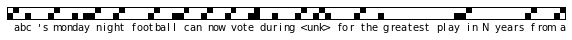
\includegraphics[scale=0.75]{chapters/COLING/schedule2} \\

\includegraphics[scale=0.75]{chapters/COLING/schedule3}
\end{tabular}
\caption{Segmentation examples. Black means $z_t=1$, white $z_t=0$.}
\label{fig:nolay}
\end{figure}

\begin{figure}[ht]
\centering
\begin{tabular}{c}

\includegraphics[scale=0.75]{chapters/COLING/layernorm} \\
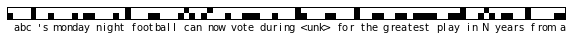
\includegraphics[scale=0.75]{chapters/COLING/layernorm2} \\

\includegraphics[scale=0.75]{chapters/COLING/layernorm3}
\end{tabular}
\caption{Segmentation examples with layer normalization. Black means $z_t=1$, white $z_t=0$.}
\label{fig:lay}
\end{figure}

The HMLSTM model predicts binary boundary variables $z^1_t$ and $z^2_t$ at each time-step, which correspond to a segment of the input utterance at each level. 
The frequencies of $z^1_t$ and $z^2_t$ provide a high-level description of segmentation properties of the network and are reported in Table~\ref{tab:ablation}. Based on the hierarchical multiscale intuition, the expected behavior is that the $z^1_t$ frequency is higher than $z^2_t$ as the former corresponds to words or morpheme-like units, whereas the latter corresponds to larger chunks. The ratio of  $z^1_t$ to $z^2_t$ frequencies is reported in the last column of Table~\ref{tab:ablation}.

Running the HMLSTM default configuration with added layer-normalization and learning-rate schedule results in the largest separation in the time-scale of the layers as indicated by the $z$-ratio of 4.67. Interestingly, only changing the $\alpha$ value to 0.125 or 0.25 results in a much narrower gap (1.78 and 1.48 respectively), without a big impact on bpc. Furthermore, the HMLSTM with schedule, layer-norm and $\alpha=0.125$ in row 5 performs on the same level as our NoTopDown ablation architecture, with a smaller $z$-ratio.

The segmentation examples reported in the original paper show the first layer of the HMLSTM segmenting the sequence at word boundaries (i.e.\ spaces), and the higher layer segments corresponding to multi-word chunks. Figure~\ref{fig:nolay} shows segmentation results of the HMLSTM with learning-rate schedule and Figure~\ref{fig:lay} with the added layer normalization.  Our runs could not reproduce the segmentation results visualized in the original paper and overall we do not find a relationship between the performance of the model and segmentation behavior.


%\section{Discussion}
%\todo{AA: There is nothing here that cannot be moved to Conclusion; I'd get rid of this section.}
%Layer-norm improved the performance by a significant margin, but only when applied at the right nodes of the computation graph. We advise to include implementation details regarding the place of application of normalization (layer-norm, batch-norm), regularization (dropout) or any other functions on otherwise well specified architectures. As noted by \cite{wilson2017marginal} adaptive methods such as Adam have emerged as popular methods as they show fast initial convergence and require little etc. However, they tend to lead to worse generalization performance than SGD with a well tuned learning-rate. In our experiments the learning-rate schedule had a large impact on the overall performance highlighting the shortcoming of vanilla Adam and the importance of running experiments with various optimization schemes. When re-applying the HMLSTM architecture to novel tasks and data sets it seems crucial to explore different optimization strategies such as switching or interpolating between adaptive methods and vanilla SGD \cite{wu2016google,akiba2017extremely,keskar2017improving}. %Running the HMLSTM with learning-rate schedule and layer-norm resulted in 1.28 bpc on PTB in our best run, but diverged at Epoch 5 in the worst case. As such, the bulk of the time in the reproduction study was devoted to find the source of the instability: different versions of tensorflow, different hardware/software setups, bugs in the source code. Our efforts were inconclusive, furthermore the authors have similar experience with such unstable behavior in other domains and models such as Relational Networks for visual reasoning or recurrent models for multi-modal speech processing. We cannot provide a conclusive solution here, but only advocate the mentioning of such instabilities in the Appendix and the measures that were taken for solving it. For example \cite{joulin2015inferring} point out that their model is sensitive to initial conditions when inferring more complex algorithmic patterns and detail the search strategy they applied in the supplementary material.

\section{Conclusion}
In our attempt to reproduce the results in \cite{chung2016hierarchical} 
we re-ran the HMLSTM model on two datasets: PTB and Text8. On PTB the 
final performance of the model almost matches the original results, 
but not quite. Our best result was achieved by a slight modification 
to the COPY operation of the last-layer provided in the source-code, 
but not detailed in the paper and with our added simplification to 
the output layer. 

We could not reproduce the results on Text8 using the same code base 
received from the authors. This might be due to the non-availability 
of the pre-processed version of the dataset. Another potential source 
might be the lack of detail in the paper on the initialization scheme 
and weight penalty, which led us to keep these implementation details 
constant across datasets. Furthermore, the layer normalization might 
have been implemented on different layers across different datasets. 
We have made several attempts until reaching the conclusion that it 
needs to be implemented on every layer of the HMLSTM. This was found 
to perform best on PTB, but might not be the best setting for Text8. 
Similarly, the learning-rate schedule was applied based on the monitoring 
of the loss after every epoch, but this was an informed guess. 

Two simplifications were applied to the architecture successfully: 
1) removing top-down connections only slightly degraded performance, and 
2) simplifying the output layer improved performance in our experiments. 
There is space for possible modifications that fell out of the scope 
of the current work like applying REINFORCE gradients in place of 
the straight-through estimator.   

We could not reproduce the segmentation results provided in the paper. 
Furthermore, we did not observe a close relationship between the segmentation 
behavior and the final performance. Changing the slope variable $\alpha$ 
to 0.25 from 0.5, while keeping all other details constant, resulted in the 
same performance, but huge difference in segmentation behavior.

The observations made here are not specific to the work of 
\cite{chung2016hierarchical} and the HMLSTM architecture. Similar results 
have been reported recently by \cite{williams2017learning}, whose 
re-implementation of the considered architecture did not produce the 
reported performances. One of their considered models learned a 
qualitatively different latent structure than another re-implementation 
by \cite{yogatama2016learning} and the other architecture did not converge 
to the same structure across runs. The HMLSTM architecture was considered 
for reproduction due to its intriguing property of learning interpretable 
structure from character-level input. The detailed reproduction and ablation 
study was provided to surface some of the potential difficulties that can 
hinder the applicability of such models for future studies. 

%\section{Acknowledgements}
%We thank Junyoung Chung for assisting us with this reproduction study of his architecture. Thanks to NWO  Aspasia grant which has funded the first author, and thanks to Microsoft, specifically Microsoft Research Montreal, for the resources.

%\bibliographystyle{acl_natbib}
%\bibliography{chapters/COLING/refs.bib}
\clearpage
\appendix
\section{Vectorized formulation of the HMLSTM}
\label{sect:appendix:vectorized_HMLSTM}

Here are the vectorized equations for the bottom, middle and top layers of the HMLSTM. Note, the computation process should be executed from top to bottom and left to right when there are multiple equations.

\subsection*{Bottom layer}
\begin{equation}
   \mathbf{c}_t = (1 - z_{t-1}) \mathbf{c}_{t-1} \odot \sigma (\mathbf{f}_t) + \text{tanh}(\mathbf{u}_t) \odot \sigma (\mathbf{i}_t) 
\end{equation}

\subsection*{Top layer}
\begin{equation}
\begin{aligned}[c]
\mathbf{\hat{c}}_t &:= \mathbf{c}_{t-1} \odot \sigma (\mathbf{f}_t) + \text{tanh}(\mathbf{u}_t) \odot \sigma (\mathbf{i}_t) \\
 \mathbf{c}_t &:= z_{t} \mathbf{\hat{c}}_t + (1 - z_t)  \mathbf{c}_{t-1}  \\
\end{aligned}
\qquad
\begin{aligned}[c]
\mathbf{\hat{h}}_t &:= \sigma (\mathbf{o}_t) \odot \text{tanh}(\mathbf{c}_t) \\
\mathbf{h}_t &:= z_{t} \mathbf{\hat{h}}_t + (1 - z_t) \odot \mathbf{h}_{t-1}
\end{aligned}
\end{equation}

\subsection*{Middle layer}
\begin{equation}
\begin{aligned}[c]
\mathrm{c}_m &= (1 - z^\ell_{t-1})   (1 - z^{\ell-1}_t) \\
\mathrm{u}_m &= (1 - z^\ell_{t-1})   z^{\ell-1}_t \\
\mathbf{u}_g &= \sigma(\mathbf{i_t}) \odot \mathrm{tanh}(\mathbf{u_t})
\end{aligned}
\qquad
\begin{aligned}[c]
\mathbf{c}_t &= \mathbf{u}_g + \mathrm{c}_m(\mathbf{c}_{t-1} - \mathbf{u}_g) + \mathrm{u}_m (\sigma(\mathbf{f_t}) \odot \mathbf{c}_{t-1}  ) ) \\
 \mathbf{h}_t &:= \sigma (\mathbf{o}_t) \odot \mathrm{tanh}(\mathbf{c}_t) \\
\mathbf{h}_t &:= \mathrm{c}_m  \mathbf{h}_t + \mathrm{c}_m \odot \mathbf{h}_{t-1}
\end{aligned}
\end{equation}
\paragraph{} Variables $\mathrm{c}_m, \mathrm{u}_m$ and $\mathbf{u}_g$ stand for copy-mask, update-mask and gated-candidate activation respectively.


\section{Vectorized formulation of the HMRNN}
\label{sect:appendix:vectorized_HMRNN}

Here are the vectorized equations for the bottom, middle and top layers of the HMRNN. Note, the computation process should be executed from top to bottom and left to right when there are multiple equations.

\paragraph{Bottom layer}
\begin{equation}
\mathbf{h}_t = \text{tanh}(W \mathbf{x}_t + (1-z^l_{t-1}) U \mathbf{h}^{l}_{t-1} + z^l_{t-1} \times V\mathbf{h}^{l+1}_{t-1})
\end{equation}

\paragraph{Top layer}
\begin{equation}
\mathbf{h}_t = (1-z^{l-1}_t) \times \mathbf{h}_{t-1} + z^{l-1}_t \times  \text{tanh}(W \mathbf{x}_t +  U \mathbf{h}^{l}_{t-1})
\end{equation}

\paragraph{Middle layer}
\begin{equation}
\begin{aligned}[c]
\mathrm{c}_m &= (1 - z^\ell_{t-1})  (1 - z^{\ell-1}_t) \\
\mathrm{u}_m &= (1 - z^\ell_{t-1})   z^{\ell-1}_t \\
\mathbf{h}_t &=  \mathrm{c}_m  \mathbf{h}_{t-1} + (1-\mathrm{c}_m)  \text{tanh}((1-\mathrm{u}_m)  \mathrm{h}_f + \mathrm{u}_m \mathrm{h}_u )) \\
\end{aligned}
\begin{aligned}[c]
\mathrm{h}_f &= W \mathbf{h}^{l-1}_t + V \mathbf{h}^{l+1}_{t-1}\\
\mathrm{h}_u &= W \mathbf{h}^{l-1}_t + U \mathbf{h}^{l}_{t-1} \\
\end{aligned}
\end{equation}
\paragraph{} Variables $\mathrm{c}_m$ and $\mathrm{u}_m$ stand for copy-mask and update-mask activation respectively.


%\end{document}

%%% Local Variables:
%%% mode: latex
%%% TeX-master: t
%%% End:
